\documentclass[12pt]{article}
\usepackage[margin=1in]{geometry} %1 inch margins
\usepackage{verbatim} %multi-line comment
\usepackage{graphicx} %graphics
\usepackage{fancyhdr} %custom header
\usepackage{amsmath} %math
\usepackage{amssymb} %math symbols
\usepackage{bm} %bold math text
\usepackage{bbm} %indicators
\usepackage{soul} %for underlining
\usepackage{listings}
\usepackage{booktabs}
%\pagenumbering{gobble} %no page numberings
\pagestyle{fancy}
\newcommand{\indep}{\raisebox{0.05em}{\rotatebox[origin=c]{90}{$\models$}}}
\allowdisplaybreaks

\renewcommand{\headrulewidth}{0pt}
\lhead{CS 208 - Applied Privacy for Data Science\\Harvard University}
\rhead{Huang, Jason\\Homework 1}
%%%%%%%%%%% BEGIN DOCUMENT
\begin{document}
\begin{center}
	{\Large \textbf{CS 208 - Applied Privacy for Data Science}}\\
	{\Large \textbf{Homework 1}}\\
	\vspace*{0.1in}
	Jason Huang\\
	Spring 2019 - Harvard University\\
\end{center}

The public Github repo containing all of the work is at https://github.com/TurboFreeze/cs208hw. All code has also been included in the appendix of this PDF as specified.

{\large\textbf{Problem 1}}

%Looking back at Latanya Sweeney's record linkage reidentification attack, she used \texttt{zip code}, \texttt{date of birth}, and \texttt{gender} to uniquely identify a large portion of the population.

The dataset was loaded into \texttt{R}, where preliminary data exploration took place. Most notably, there are 25766 entries and 18 variables in the dataset, with the variables being:
\begin{center}
\texttt{state, puma, sex, age, educ, income, latino, black, asian, married, divorced, uscitizen, children, disability, militaryservice, employed, englishability, fips}
\end{center}
The naive and most effective starting point is tallying the unique values for each of these variables. Two of the variables, \texttt{state} and \texttt{fips}, have the same value for all rows and therefore will not be considered at all.

%\texttt{serialno.household} is a household identifier that is likely not easily available publicly and/or unlikely to exist in a third-party source for cross-referencing. If it was available, then it alone would be sufficient to uniquely identify the vast majority of individuals. Note that household identifier has a flexible range, meaning that a larger sample likely includes more serial numbers (unlike other attributes like age), and therefore despite being a 5\% sample, it has a similar distribution as the entire population. Since there are 973 unique household serial numbers in this sample of 1000, then roughly 97\% of individuals can be uniquely identified based on this identifier alone, on the assumption that it exists in a cross-reference database. These calculations are just to demonstrate a basic sample calculation of an effective identifier, but since it is unlikely to be available, as has already been stated, it will be disregarded from this point onward.

%Examining location identifiers, the question implies the inclusion of \texttt{puma}. Examining the rest of the variables, note that  \texttt{puma} = \texttt{jpumarow} + 1090 and \texttt{puma} = \texttt{X} + 566, meaning that it provides absolutely no unique information beyond what is already known from \texttt{puma} and can thus be ignored. 
%%%
%The approach that will then be used is as follows: \emph{examine the entire 5\% sample across all PUMA regions, extrapolate to the entire population by multiplying by 20, and then divide by 7 to achieve the final result due to the assumption that there are 7 roughly uniformly sized PUMA regions in the provided data sample}.

%Since a worst-case lower bound is always safer than overestimating, this will be the process used here.
Now examine the most identifying variables (i.e. the variables with most unique values in the dataset, as determined by taking the length of its count table in \texttt{R}).
\begin{center}
\begin{tabular}{||c|c|c|c||}
\hline
\texttt{income} & \texttt{age} & \texttt{educ} & \texttt{puma} \\\hline
2763 & 73 & 16 & 7 \\ \hline
\end{tabular}
\end{center}
All the other variables are binary variables (can only have two distinct values). \texttt{puma} is implicitly included (since the goal is to uniquely identify individuals \emph{within a PUMA region}) and will be accounted for in the last step. However, these other three variables should be explored, particularly by examining their distributions, as plotted below.

\begin{center}
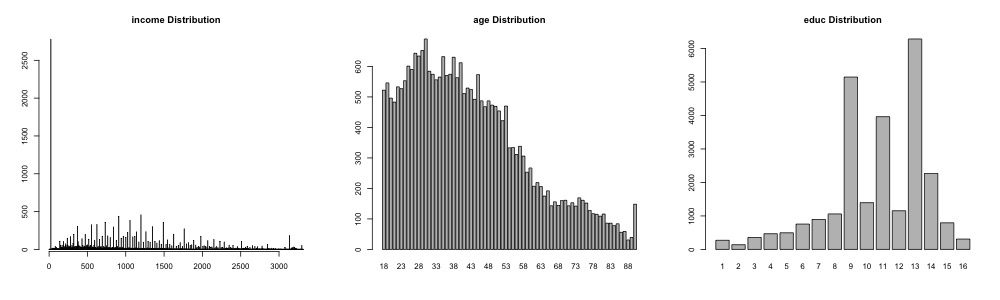
\includegraphics[width=\textwidth]{figs/exploredist}
\end{center}

The goal now is to quantify exactly how identifiable each variable is. Estimates for the probability of collision (of another individual having the exact same value) for each variable based on the largest bin (i.e. worst case) are made below. Actual probabilities for collision can also be calculated by the following formula:
\[p_{collision}=p(X_1 = X_2) = \sum\limits_{x} p(X_1 = x)p(X_2=x) = \sum\limits_x \left(\dfrac{\text{count}(x)}{25766}\right)^2\]
where $x$ is to take on all possible values for that variable.

\texttt{income} is the most identifiable variable but also raises an issue when examining the distribution histogram: a large number of individuals have zero income, and are therefore substantially more difficult to uniquely identify. Apart from this unique case, though, no bin has more than 500 individuals, which corresponds to approximately 500/25766 $\approx$ 2\% of collision with another individual (actual: {0.01555964}). \texttt{age} is distributed a lot better, with the worst case bin having no more than 800 individuals with the same age. When considering the overall size of 25766, that means that there is \emph{at most} a 800/25766 $\approx$ 3\% chance of having the same age as a randomly chosen person in the dataset (actual: {0.01831928}). Lastly, for \texttt{educ}, with up to 6500 in the same bin, the probability of having the same education level as someone else would be 6500/25766 $\approx$ 25\% (actual: {0.1416453}).

Percentage estimates where given above to provide intuition and also as a sanity check, but the actual values calculated will be the ones used from here on.

When taking these three variables together, the probability of the collision is the intersection of all three variables colliding, which is the product of the three probabilities. This gives an overall probability of colliding to be $0.01555964 \times 0.01831928 \times 0.1416453 \approx \textbf{0.00004} = p_{collision}$.

Now, the geographic identifier of PUMA regions needs to be taken into account. Here is a summary of counts for each PUMA region.
\begin{center}
\begin{tabular}{|c|ccccccc|}
\hline
\textbf{PUMA} & 1101 & 1102 & 1103 & 1104 & 1105 & 1106 & 1107\\\hline
\textbf{Count} & 3215 & 5736 & 3728 & 3740 & 3128 & 3236 & 2983\\ \hline
\end{tabular}
\end{center}
These are very roughly equal (i.e. on the same order of magnitude), and these do appear to be 5\% samples (with full populations of ~50000-120000 in each PUMA, which is appropriate). Assume the average PUMA region to therefore be 1/7 of the total dataset: $(1/7) \times 20 \times 25766 = 73617$.

To finally determine the percentage of individuals $p(U)$ within a PUMA that can be uniquely identified by the aforementioned variables, this calculation simply involves the probability of no collision with anyone in that region of size $n$, or:
\[p_{unique} = (1-p_{collision})^{n}\]

In this situation, $p_{collision} = 0.00004, n = 73617$ as calculated above, so:
\[p_{unique} = 0.051183922689063\]

$\therefore$ With the three variables of \texttt{income}, \texttt{age}, \texttt{educ}, approximately $\boxed{5\%}$ of the population within a single PUMA can be identified.

Better reconstruction results can be achieved using more variables. The only remaining variables are binary, which should have roughly 50\% chance of collision (though in actuality it will be higher due to uneven distribution). The lowest probabilities of collision are for \texttt{sex} (0.5014973) and \texttt{married} (0.5046546), two common and relatively evenly distributed binary indicators. When factoring these in, then:
\[p_{collision} = 0.00001 \implies p_{unique} = 0.471312198919265\]
$\therefore$ With the five variables of \texttt{income}, \texttt{age}, \texttt{educ}, \texttt{sex}, \texttt{married}, approximately $\boxed{47\%}$ of the population within a single PUMA can be identified.

While it is more difficult and less likely to orchestrate a reconstruction attack with large numbers of variables, out of interest and completeness, here are some further results. With a sixth variable of \texttt{black}, 68\% of the population can be uniquely identified. With a seventh added variable of \texttt{employed}, 81\% of the population can be uniquely identified. The remaining binary variables have sharply decreasing utility due to their uneven distribution (i.e. almost all individuals have the same value and therefore it is not very helpful in identifying someone).

Finally, some small disclaimers. The results above are all approximate and derived from rough back-of-the-envelope calculations. They are also assuming that these variables are available in external sources for cross-referencing, which may present practical obstacles that may or may not be easy to handle. For example, a specific education encoding is used here. Other government databases may use the same schema, making cross-referencing trivial. Furthermore, knowing an individual's exact education level may also be sufficient to map it to one of the factors in this dataset's \texttt{educ} schema. However, if a different, less granular schema was used (i.e. only 5 levels instead of 16), then cross-referencing may not really be possible. Different levels of granularity would be a particularly common issue for \texttt{income}, with added concerns such as rounding. It may also affect \texttt{age}, though probably to a much lesser extent. Binary variables should otherwise be less problematic in this regard.\\
\pagebreak

{\large\textbf{Problem 2}}

The code for this problem can be found in \texttt{q2reconstruction.R}. In this problem, a reconstruction attack was executed against three defense mechanisms (rounding, noise, subsampling) in a \texttt{R} script. Plots of the results follow, with the parameter values for each defense ranging from 1 to $n$ (note that it is not really possible to round to the nearest multiple of 0, nor subsample 0 out of $n$ rows). The resulting fraction of results that were successfully reconstructed were plotted against the root-mean-squared error (RMSE) metric. Each data point is the average of 10 trials in order to account for the randomness introduced by the defense mechanisms.
\begin{center}
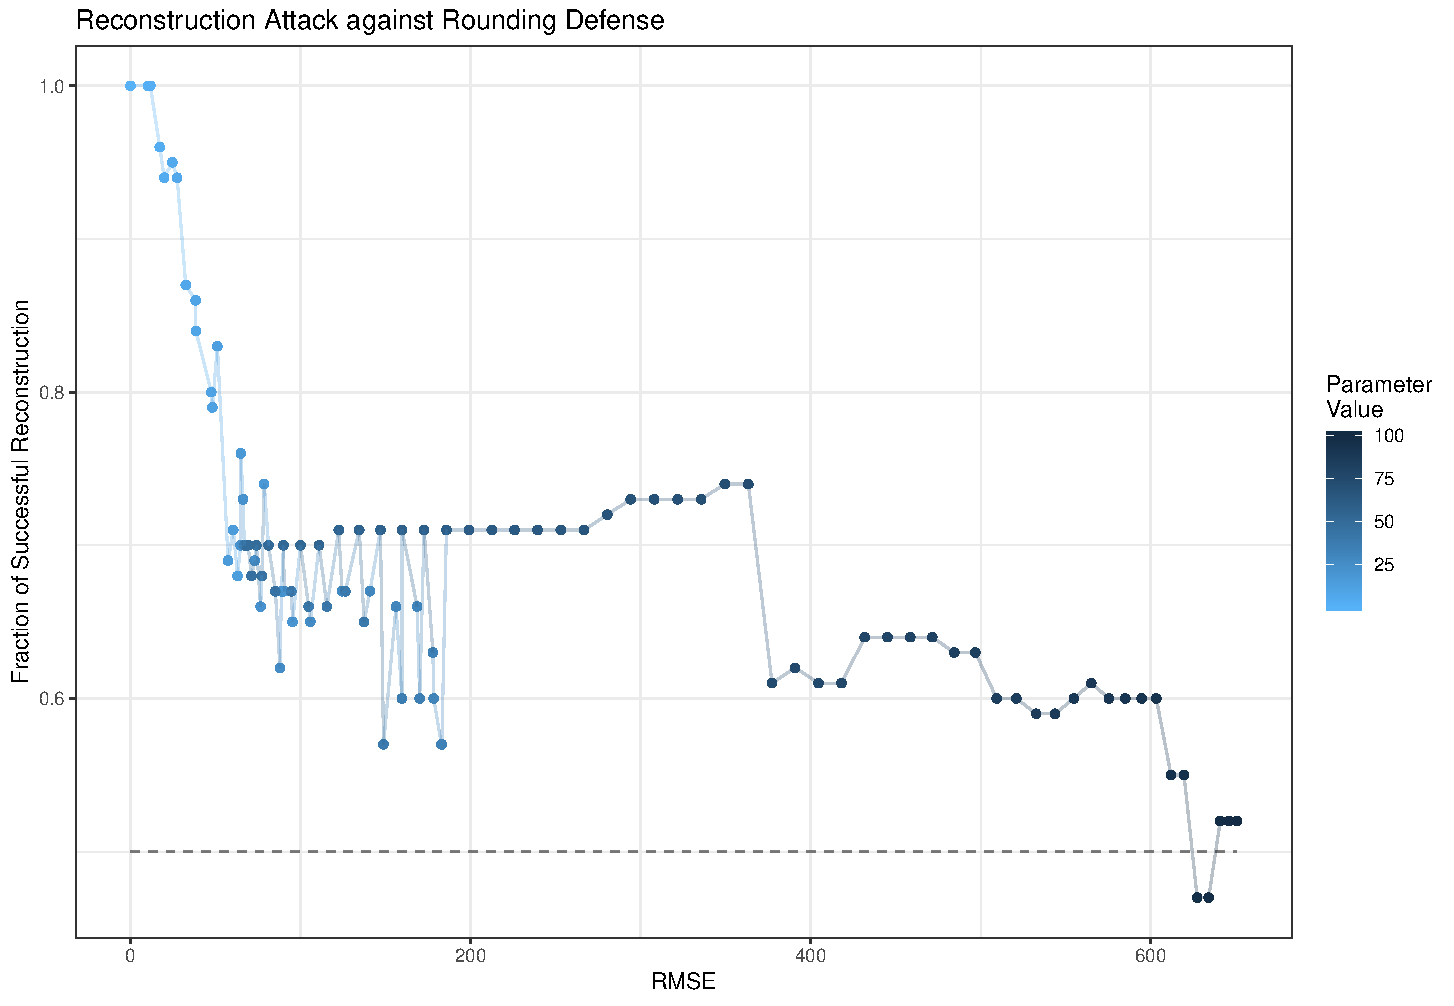
\includegraphics[width=\textwidth]{figs/attackrounding}
\end{center}
With the above attack against the rounding defense, the first failure occurs with $R = 15$ and the last success occurs at $R = 25$. The reconstruction fraction declines rapidly before oscillating substantially just below the success threshold.

\begin{center}
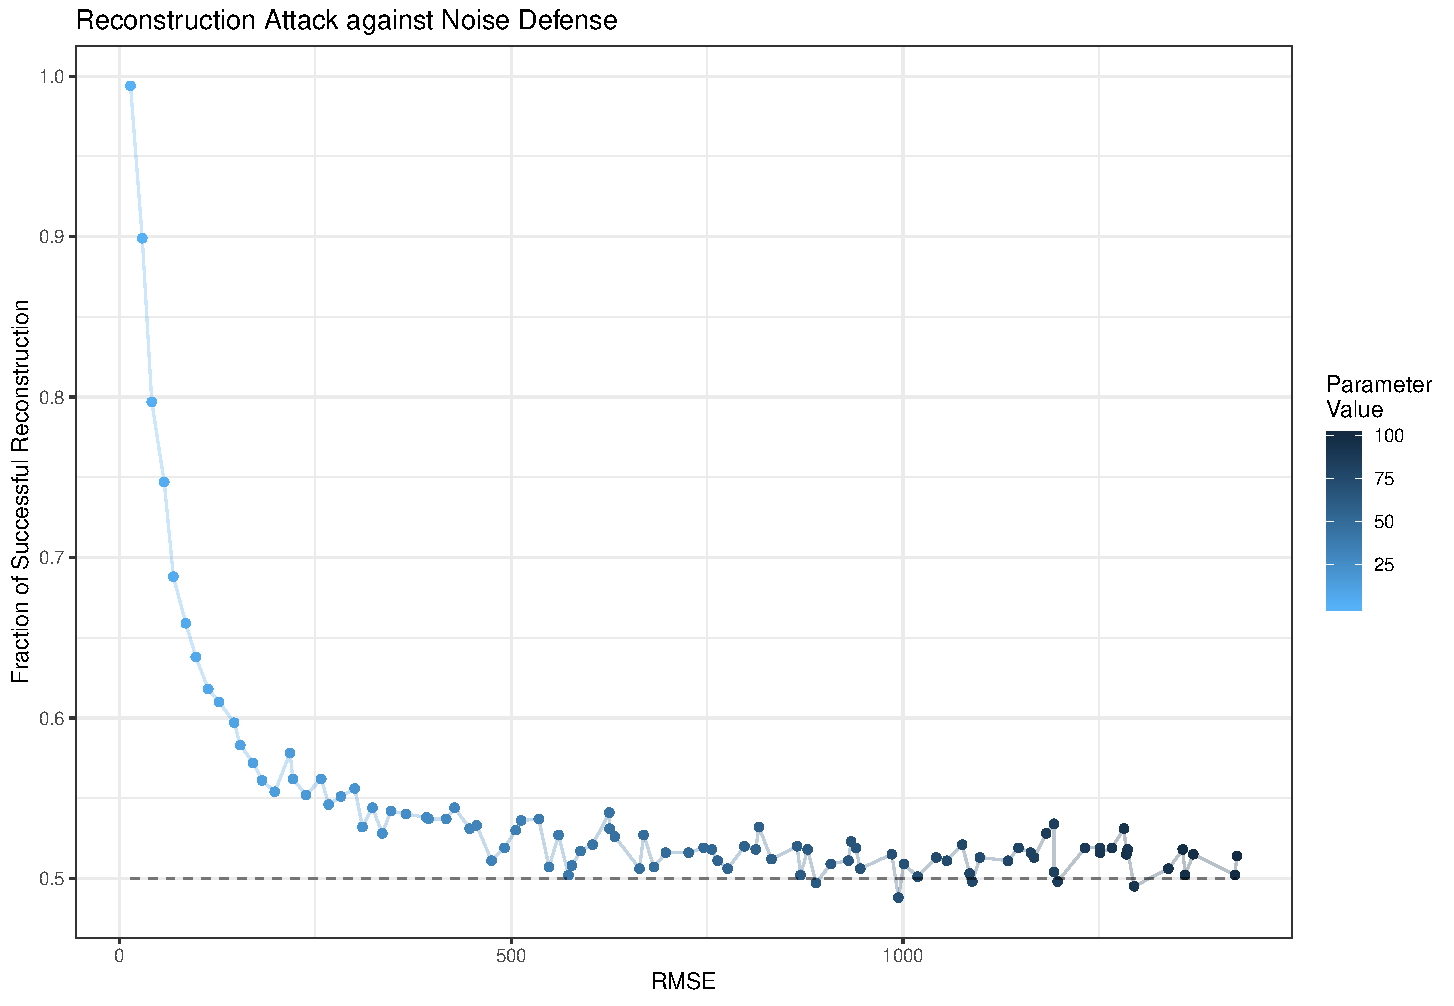
\includegraphics[width=\textwidth]{figs/attacknoise}
\end{center}
With the above attack against the noise injection defense, the results drop precipitously and clearly cross from success to failure with all $\sigma > 3$ producing high enough noise to result in failure.

\begin{center}
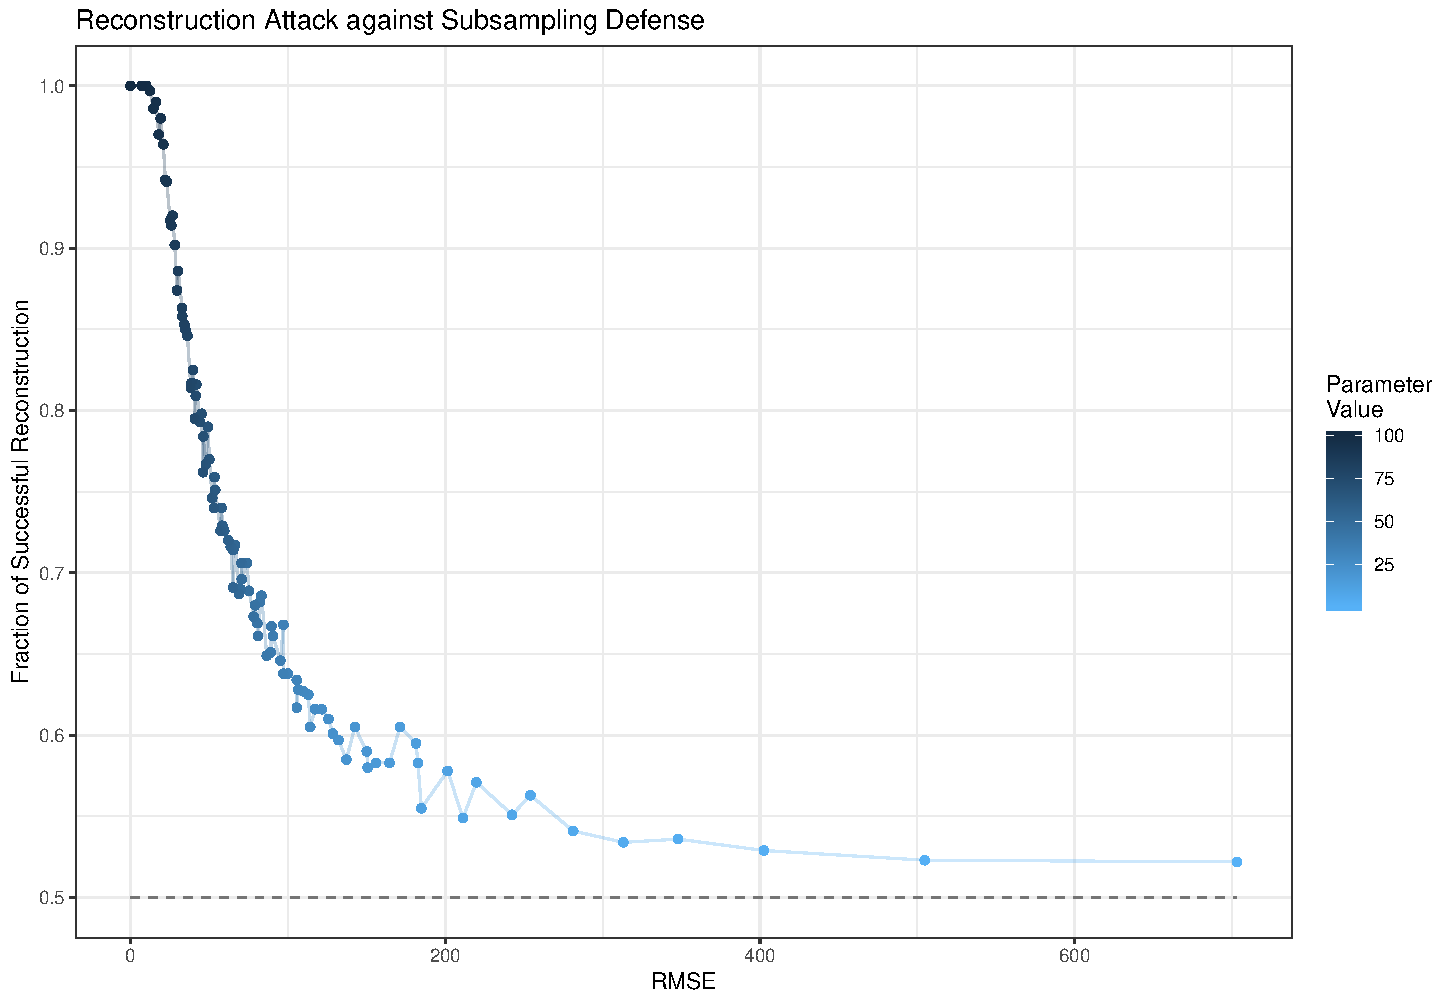
\includegraphics[width=\textwidth]{figs/attacksubsampling}
\end{center}
For the subsampling defense, larger subsamples result in worse privacy, with anything above subsamples of size 64 providing sufficient protection against successful reconstruction.
\pagebreak

{\large\textbf{Problem 3}}

\pagebreak

{\large\textbf{Problem 4}}



{\large\textbf{Appendix}}

\textbf{Code for Problem 1}
\begin{lstlisting}[language=R]
##
## q1.r
##
## Exploring Fulton PUMS data to identify variables for reidentification attack 
##
## JH 2019/02/11
##

# read in the data
data <- read.csv('FultonPUMS5full.csv')
# summary of data
head(data)
nrow(data)
# variables
print(paste(names(data), collapse=", "))
print(length(names(data)))

# see how many unique values of each variable
vars <- c()
counts <- c()
for (n in names(data)) {
  vars <- c(vars, n)
  counts <- c(counts, nrow(unique(data[n])))
}
results <- data.frame(var=vars, count=counts)

# look at location identifiers
table(data$puma)
# unique(data$puma - data$jpumarow)
# unique(data$puma - data$X)
# # remove duplicates
# results <- results[!results$var %in% c("X", "jpumarow"),]

# remove variables with single count
results[results$count == 1,] # state and fips have one count
results <- results[results$count != 1,]


# plot distributions
jpeg('./figs/exploredist.jpg', width=1000, height=300)
par(mfrow=c(1,3))
barplot(table(data$income), xaxt='n', ylab='', main="income Distribution")
axis(side=1)
barplot(table(data$age), ylab='', main="age Distribution")
barplot(table(data$educ), ylab='', main="educ Distribution")
par(mfrow=c(1,1))
dev.off()


# collision probabilities
collision <- function(vardata) {
  sum((table(vardata) / nrow(data))^2)
}

p.collisions <- c()
for (v in as.character(results$var)) {
  p.collisions <- rbind(p.collisions, c(v,collision(data[v])))
}
p.collisions

# find average size of PUMA
avg.puma <- round(20 * nrow(data) / length(unique(data$puma)))

# calculate joint probability of collision
collision.joint <- function (vars) {
  joint <- 1
  for (v in vars) {
    joint <- joint * collision(data[v])
  }
  joint
}

# calculate percentage of average PUMA uniquely identifiable
identifiable <- function (p.collision) {
  (1 - p.collision)^avg.puma
}


# calculate results with proposed list of identifying variables
varlist <- c("income", "age", "educ")
identifiable(collision.joint(varlist))
varlist <- c(varlist, "sex", "married")
identifiable(collision.joint(varlist))
varlist <- c(varlist, "black")
identifiable(collision.joint(varlist))
varlist <- c(varlist, "employed")
identifiable(collision.joint(varlist))
\end{lstlisting}

\pagebreak

\textbf{Code for Problem 2}

\begin{lstlisting}[language=R]
##
## q2reconstructionattack.r
##
## Regression-based reconstruction attack against various defense mechanisms
##
## JH 2019/02/21
##

library(ggplot2)    # using ggplot graphing libraries (optional)

##### Parameters

set.seed(99)          # RNG seed
n <- 100              # Dataset size
k.trials <- 2 * n     # Number of queries
exp.n <- 10           # Number of experiments at each step

##### Data

# read in the data
sample.data <- read.csv('FultonPUMS5sample100.csv')
sample.data.clean <- sample.data[3:17]
attributes.n <- length(names(sample.data.clean))

# get sensitive data (USCITIZEN)
sensitive.var <- "uscitizen"
sensitive.data <- sample.data[, sensitive.var]


##### Querying Mechanisms (including defenses)

# standard query of the dataset
query <- function(data, pred) {
  # extract data subset according to specified predicate
  subset <- data[pred]
  # calculate desired sum
  sum <- sum(subset)
  sum
}

# query w/ defense by rounding to nearest multiple of R
query.rounding <- function(data, pred, r) {
  # get actual query
  sum <- query(data, pred)
  # apply rounding defense
  sum.rounded <- round(sum / r) * r
  sum.rounded
}

# query w/ defense by adding Gaussian noise
query.noisy <- function(data, pred, sigma) {
  # get actual query
  sum <- query(data, pred)
  # apply Gaussian noise as defense
  sum.noisy <- sum + rnorm(1, 0, sigma)
  sum.noisy
}

# query w/ defense by subsampling t out of n rows
query.subsampling <- function(data, pred, t) {
  # create subsample T with t out of n rows
  T.rows <- sample(length(data), t)
  # extract data subset from subsample according to specified predicate
  T.data <- data[T.rows]
  # get actual query on this subsample
  sum <- query(T.data, pred[T.rows])
  # scale up
  sum.sub <- sum * length(data) / t
  sum.sub
}


##### Define Predicates

# hashing to generate predicates
prime <- 563    # moderately large prime

predicate.single <- function(r.nums, individual) {
  (sum(r.nums * individual) %% prime) %% 2
}

# define predicates for the 2n queries
predicates <- matrix(NA, nrow = k.trials, ncol = n)

# generate 2n predicates
for (pred.index in 1:k.trials) {
  # generate random numbers for this hash
  r.nums <- sample(0:(prime - 1), attributes.n, replace=TRUE)
  # calculate for particular individual
  pred.temp <- apply(sample.data.clean, MARGIN = 1, predicate.single, r.nums)
  # store the predicate
  predicates[pred.index,] <- pred.temp
}


#### Main Reconstruction Attack function
# takes a defense query mechanism and name of defense
# makes the attack and plots the results
reconstruction <- function (query.function, defense.name) {
  results <- data.frame(param=integer(), rmse=numeric(), frac=numeric())
  # loop through different parameter values
  for (param.value in 1:n) {
    # make 10 experiments each time, storing each RMSE and fraction of success
    experiments.rmse <- vector("numeric", exp.n)
    experiments.frac <- vector("numeric", exp.n)
    for (exp.index in 1:exp.n) {
      squared.errors <- c()
      history <- matrix(NA, nrow = k.trials, ncol = (n + 1))
      
      ##### Run Queries
      # make the 2n queries using the generated predicates
      for (pred.index in 1:k.trials) {
        # extract predicate
        pred.current <- predicates[pred.index,]
        # get standard query and query with defense
        q.standard <- query(sensitive.data, pred.current)
        q.defense <- query.function(sensitive.data, pred.current, param.value)
        # save this query (result w/ defense + predicate) to history table
        history[pred.index,] <- c(q.defense, as.numeric(pred.current))
        # calculate and store squared errors
        squared.errors <- c(squared.errors, (q.defense - q.standard) ** 2)
      }
      # calculate RMSE for this experiment
      experiments.rmse[exp.index] <- sqrt(sum(squared.errors))
      
      # convert into dataframe
      xnames <- paste("x", 1:n, sep="")
      varnames <- c("y", xnames)
      release.data <- as.data.frame(history)
      names(release.data) <- varnames
      
      ##### Regression Attack
      # attack formula
      attack.formula <- paste(xnames, collapse=" + ")
      attack.formula <- paste("y ~ ", attack.formula, "-1")
      attack.formula <- as.formula(attack.formula)
      attack.output <- lm(attack.formula, data=release.data)
      # regression coefficient estimates
      attack.estimates <- attack.output$coef
      # estimates rounded to give reconstruction predictions
      attack.reconstructed <- round(attack.estimates)
      # calculate fraction successfully reconstructed
      experiments.frac[exp.index] <-
        sum(attack.reconstructed == sensitive.data) / n
    }
    # append the avg of the 10 experiments for this particular parameter value
    results <- rbind(results,
                     c(param.value, mean(experiments.rmse), mean(experiments.frac)))
  }
  
  names(results) <- c("param", "rmse", "frac")
  
  ##### Visualization of results
  # type to distinguish between successful (1) or not (0)
  results$success <- as.numeric(results$frac > 0.5)
  print(paste("Min:", min(results[results$success == 0,]$param)))
  print(paste("Max:", max(results[results$success == 0,]$param)))
  # plot the result
  ggplot(results, aes(x=rmse, y=frac)) + # scatter plot
    geom_point(aes(color=param, shape=as.factor(success + 23))) + 
    # trend line
    geom_line(aes(color=param), alpha=0.3) +
    # success threshold
    geom_line(aes(y=0.5), alpha=0.5, size=0.5, linetype=2) +
    # labels and title
    ylab("Fraction of Successful Reconstruction") +
    xlab("RMSE") +
    ggtitle(paste("Reconstruction Attack against", defense.name)) + 
    # legend formatting
    scale_color_continuous(name="Parameter\nValue", low="#56B1F7", high="#132B43") +
    scale_shape_discrete(name="Outcome", labels=c("Failure", "Success")) +
    theme_bw()
  #plot(results$frac, results$rmse) # use this instead if no ggplot
}

# make the calls to the reconstruction attack function
reconstruction(query.rounding, "Rounding Defense")
dev.copy2pdf(file="./figs/attackrounding.pdf")
reconstruction(query.noisy, "Noise Defense")
dev.copy2pdf(file="./figs/attacknoise.pdf")
reconstruction(query.subsampling, "Subsampling Defense")
dev.copy2pdf(file="./figs/attacksubsampling.pdf")
\end{lstlisting}


\pagebreak

\textbf{Code for Problem 3}


\end{document}